\chapter{\textcolor{black}{Background}}
In this chapter, following subjects will be covered: theoretical background of maze-generating algorithms, maze-solving algorithms,
and other theoretical concepts from the graph theory required to better understand the problems included in this work. \textcolor{black}{Moreover the concept of determining the difficulty
of a maze will be introduced}. 
\section{Graph Theory}
In the following section, the graph theory most important mathematical concepts, and a naming convention to follow in this paper will be established. 
\begin{definition}\textbf{A Set} \emph{is an object of distinct elements where no element is a set itself\cite{5}.}\end{definition}
\begin{definition}\textbf{A Graph} \emph{is an object comprising two sets called vertex set V and edge set E. V is a finite, nonempty and the E may be empty. A graph usually denoted as $ G = (V, E)$\cite{5}.}\end{definition}
\noindent In this work, two interesting subgroups of graphs will be discussed: directed graph, and cyclic graph. By applying \textit{direction} to edges of a \textit{undirected}, \textit{acyclic} graph presented on Figure 2.1(a), we are receiving a \textit{directed graph} presented on Figure 2.1(b). A cyclic graph consists of at least one single \textit{cycle}, which means at least 3 vertices connect in a closed chain Figure 2.1(b). 
 \begin{figure}[!h]
	\centering
	\begin{subfigure}{.35\textwidth}
	  \centering
	  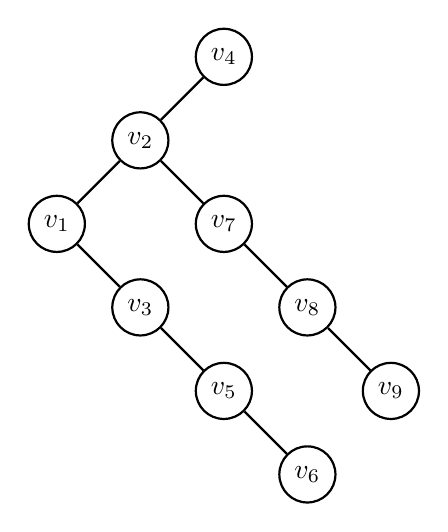
\begin{tikzpicture}[node distance={15mm}, thick, main/.style = {draw, circle}] 
		\node[main] (1) {$v_1$}; 
		\node[main] (2) [above right of=1] {$v_2$}; 
		\node[main] (3) [below right of=1] {$v_3$}; 
		\node[main] (4) [above right of=2] {$v_4$}; 
		\node[main] (5) [below right of=3] {$v_5$}; 
		\node[main] (6) [below right of=5] {$v_6$}; 
		\node[main] (7) [below right of= 2] {$v_7$};
		\node[main] (8) [below right of= 7] {$v_8$};
		\node[main] (9) [below right of= 8] {$v_9$};
		\draw (1) -- (2);
		\draw (2) -- (4);
		\draw (1) -- (3);
		\draw (3) -- (5);
		\draw (5) -- (6);
		\draw (2) -- (7);
		\draw (7) -- (8);
		\draw (8) -- (9);
		\end{tikzpicture} 
	  \caption{}
	  \label{fig:sub1}
	\end{subfigure}
	\begin{subfigure}{.35\textwidth}
	  \centering
	  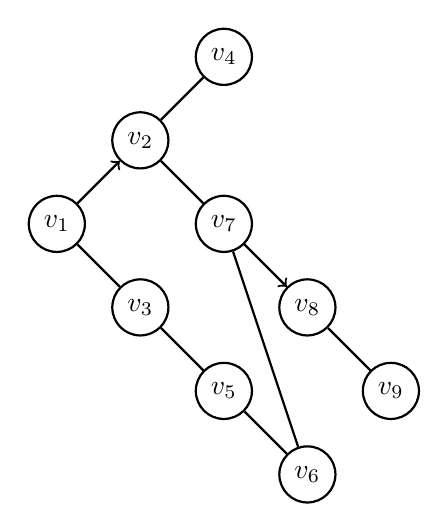
\begin{tikzpicture}[node distance={15mm}, thick, main/.style = {draw, circle}] 
		\node[main] (1) {$v_1$}; 
		\node[main] (2) [above right of=1] {$v_2$}; 
		\node[main] (3) [below right of=1] {$v_3$}; 
		\node[main] (4) [above right of=2] {$v_4$}; 
		\node[main] (5) [below right of=3] {$v_5$}; 
		\node[main] (6) [below right of=5] {$v_6$}; 
		\node[main] (7) [below right of= 2] {$v_7$};
		\node[main] (8) [below right of= 7] {$v_8$};
		\node[main] (9) [below right of= 8] {$v_9$};
		\draw[->] (1) -- (2);
		\draw (2) -- (4);
		\draw (1) -- (3);
		\draw (3) -- (5);
		\draw (5) -- (6);
		\draw (2) -- (7);
		\draw (6) -- (7);
		\draw[->] (7) -- (8);
		\draw (8) -- (9);
		\end{tikzpicture} 
	  \caption{}
	  \label{fig:sub2}
	\end{subfigure}
	\caption{In this picture different types of graphs are presented. Graph (a) is an undirected, acyclic graph, where \textit{v} denotes a vertex. Graph (b) has two directed edges marked by an arrow, and contains one cycle $x_1 \rightarrow x_2 \rightarrow x_7 \rightarrow x_6 \rightarrow x_5 \rightarrow x_3$.\\Source: developed by the author.}
	\label{fig:test}
	\end{figure}

\begin{definition} \textbf{An Adjacency Matrix } \emph{of a graph $G=(V, E)$ is a representation in which we number the vertices in some arbitrary way e.g. $1,2,3,\dots, |V|$. The representation of a Matrix of
consisting $|V|x|V|$ such that: 
$$A(i,j)=
\begin{cases}
1, \emph{if}  (i,j)\in E,\\
0, otherwise\\
\end{cases}$$
}
\\
\emph{Figures 2.2(a) and 2.2(b) are the adjacency matrices of \textcolor{black}{graphs presented on Figure 2.1(a) and 2.1(b) respectivly}.
The adjacency matrix of a graph requires $O(|V|^2)$ memory, independent of the number of edges in the graph.}
\end{definition}
\begin{figure}[!h]
	\centering
	\begin{subfigure}{.35\textwidth}
	  \centering
	  $\begin{pmatrix}
		0&1&1&0&0&0&0&0&0\\
		1&0&0&1&0&0&1&0&0\\
		1&0&0&0&1&0&0&0&0\\
		0&1&0&0&0&0&0&0&0\\
		0&0&1&0&0&1&0&0&0\\
		0&0&0&0&1&0&0&0&0\\
		0&1&0&0&0&0&0&1&0\\
		0&0&0&0&0&0&1&0&1\\
		0&0&0&0&0&0&0&1&0\\
	\end{pmatrix}$
	  \caption{}
	  \label{fig:sub1}
	\end{subfigure}
	\begin{subfigure}{.35\textwidth}
	  \centering
	  $\begin{pmatrix}
		0&1&1&0&0&0&0&0&0\\
		0&0&0&1&0&0&1&0&0\\
		1&0&0&0&1&0&0&0&0\\
		0&1&0&0&0&0&0&0&0\\
		0&0&1&0&0&1&0&0&0\\
		0&0&0&0&1&0&1&0&0\\
		0&1&0&0&0&0&0&1&0\\
		0&0&0&0&0&0&0&0&1\\
		0&0&0&0&0&0&0&1&0\\
	\end{pmatrix}$
	  \caption{}
	  \label{fig:sub2}
	\end{subfigure}
	\caption{Examples of different adjacency matrices: adjacency matrix (a) is a matrix of graph presented in Figure 2.1(a), adjacency matrix (b) is a matrix of graph in Figure 2.1(b).\\Source: developed by the author.}
	\label{fig:test}
\end{figure}

	\newpage
	\begin{definition} \textbf{Density r} \emph{of a graph defines how complete the graph is. We define density as the number of edges divided by the number called \txtit{possible}. The number of possible is the maximum number of edges that the graph can contain.
	If self-loops are excluded, then the number possible is:\\
	\begin{equation}\label{acyclic_density}
	\frac{n(n-1)}{2}
	\end{equation}
	\textbf{Where:}\\
	$n$ is the number of vertices in a graph.\\
	\newline
	If self-loops are allowed, then the number possible is:
	\begin{equation}\label{cyclic_density}
	\frac{n(n+1)}{2}
	\end{equation}
	}
	\newline
	\end{definition}
\begin{definition}\textbf{A Free Tree} \emph{ is an undirected, acyclic, connected graph. Let $G = (V,E)$ be an undirected graph. Properties of a tree \cite{6}:}\\
	$-$ \textit{G} is a free tree,\\
	$-$ every two vertices in \textit{G} are connected by a unique path,\\
	$-$ \textit{G} is connected, but if any edge is removed from \textit{E},the graph becomes disconnected,\\
	$-$ \textit{G} is connected, and $|E| = |V| - 1$,\\
	$-$ \textit{G} is acyclic, and $|E| = |V| - 1$\\
	$-$ \textit{G} is acyclic, but if we add any edge to \textit{E}, the graph contains a cycle.\\
\end{definition}
\begin{definition}\textbf{A Binary Tree} $B$ \emph{is a tree in which each vertex has no more than two subordinate vertices. It is composed of three disjoint sets of vertices: a root vertex, a binary tree called its left subtree, and a binary tree called its right subtree \cite{7}.}\end{definition}
\begin{definition}\textbf{A Spanning Tree }\textit{T} \emph{is an acyclic tree which connects all the vertices in the graph \textit{G}. The minimum-spanning problem is a problem of determining the tree \textit{T} whose total weight is minimized \cite{8}.}\end{definition}
\begin{definition}\textbf{A Path } \emph{in a graph $G$ is a sequence of vertices $v_1, v_2,\ldots,v_k$. In cyclic mazes, paths can be infinite. The shortest path is a path with the lowest cost between any two given vertices \cite{9}.}\end{definition}
\begin{definition}\textbf{A Shortest Path Problem } \emph{is finding for a given graph $G = (V,E)$, a shortest path from any 2 given nodes \textit{u} to \textit{v}. Shortest-paths algorithms typically rely on the property that the shortest path between two vertices contains other shortest paths within it.
The shortest path cannot contain any cycles \cite{5}.}\end{definition}
\begin{definition}\textbf{A Cell} \emph{is a single vertex in the maze matrix. The position of a cell is given by its $id$ eg. for a cell with a position $a_{11}$ in a grid, we will note the id as $"1\char"0023 1"$, A cell is also the smallest element of the maze. The cell keeps the following information: its coordinates, the number of neighbours and their’s position relative to the cell.}\end{definition}
\begin{definition}\textbf{A Degree } \emph{of a vertex is denoted as $d(v)$ and it describes the number of adjacent cells \cite{10}.}\end{definition}
\begin{definition}\textbf{An Average Degree }\emph{ $\bar{d}$ for a given graph is given by~\cite{10}:\\
\begin{equation}
\bar{d} = \frac{r}{n-1}	
\end{equation}
\textbf{Where:}\\
$n$ is a number of vertices in the graph\\	
}\end{definition}
\begin{definition}\textbf{A Dead End} \emph{ is defined as a node with a degree $d(v) = 1$. In the maze \textcolor{black}{it is} a cell that is linked to only one adjacent node.}\end{definition}
\begin{definition}\textbf{A Fork} \emph{is defined as a node with a degree $d(v) = 2$. In the maze, it is a cell that is linked to two adjacent nodes.}\end{definition}
\begin{definition}\textbf{An Intersection} \emph{ is defined as a node with a degree $d(v) = 3$. In the maze, it is a cell that is linked to three adjacent nodes.}\end{definition}
\begin{definition}\textbf{A Cross} \emph{is defined as a node with a degree $d(v) = 4$. In the maze, it is a cell that is linked to four adjacent nodes. }\end{definition}
\begin{definition}\textbf{A Grid} \emph{in this \textcolor{black}{thesis} is considered as a square matrix. Its size defines the size of a maze $n \times m$. The grid keeps the information about each cell and its relative positions in an array.}\end{definition}
\begin{definition}\textbf{A Move} \emph{is considered as a transition from one cell to one of its closest neighbours. In this \textcolor{black}{work}, we are using only NSWE moves presented in Figure 2.3. Diagonal moves are forbidden.
\newline
\begin{figure}[!h]
	\centering
	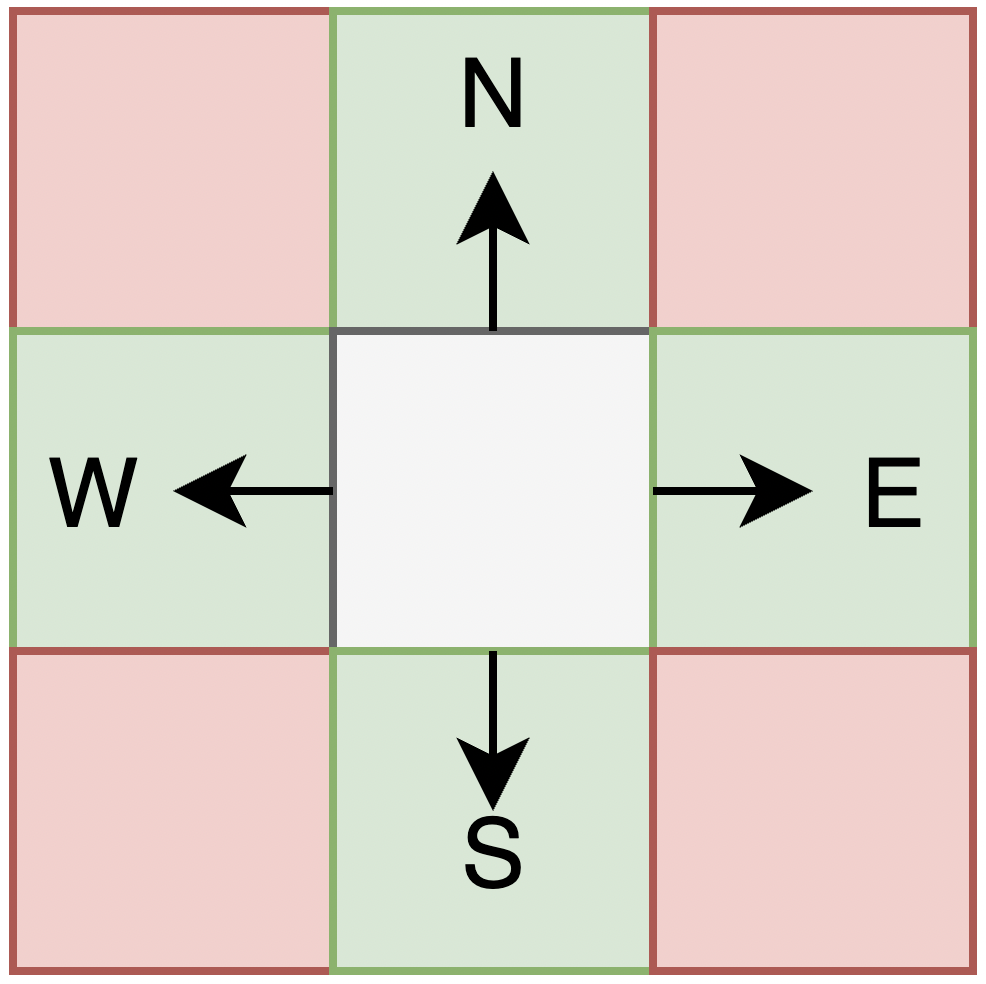
\includegraphics[width=.2\linewidth]{moves}
	\caption{Allowed moves.\\Source: developed by the author}
\end{figure}		
}\end{definition}
\begin{definition}\textbf{A Maze} \emph{can be considered as a graph, where each intersection is a vertex, and the path between them is an edge. }\end{definition}
\noindent In this thesis a few types of mazes will be considered:\\
$-$ perfect maze,\\
$-$ directed maze,\\
$-$ cyclic maze.\\
The perfect maze is a maze with only one path between any two given nodes, a directed maze is be a maze with some paths directed in a certain direction,
and a cyclic maze is be a maze with at least one cycle. Different types of mazes are presented in Figure 2.4.\\ 
 \begin{figure}[!h]
	\centering
	\begin{subfigure}{.45\textwidth}
	  \centering
	  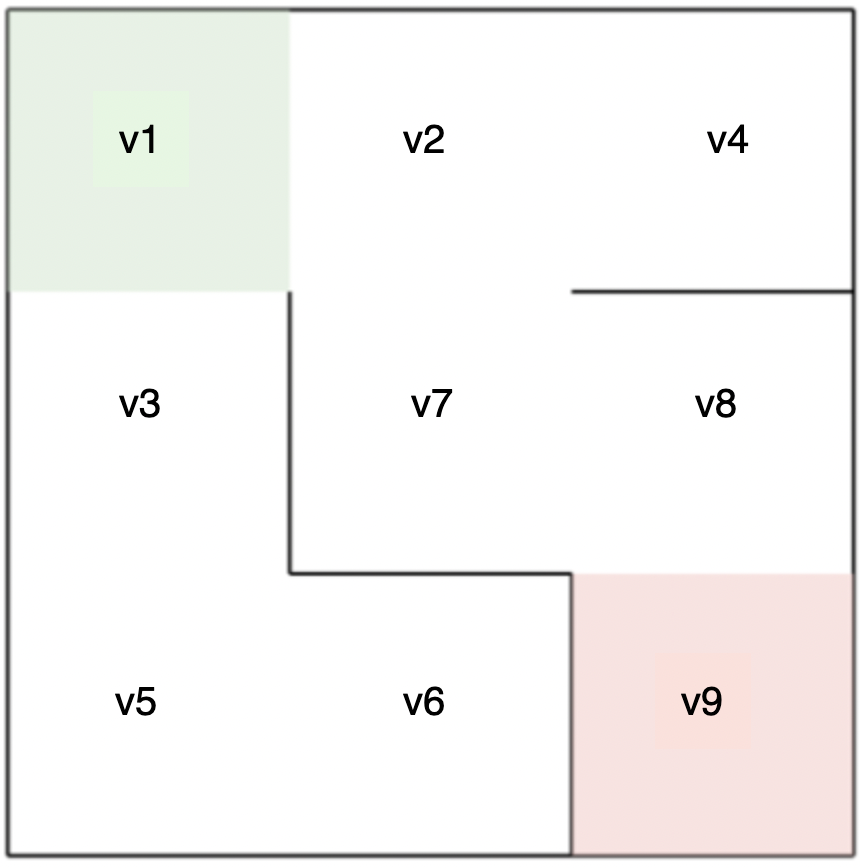
\includegraphics[width=.6\linewidth]{undirectedmaze}
	  \caption{}
	  \label{fig:sub1}
	\end{subfigure}
	\begin{subfigure}{.45\textwidth}
	  \centering
	  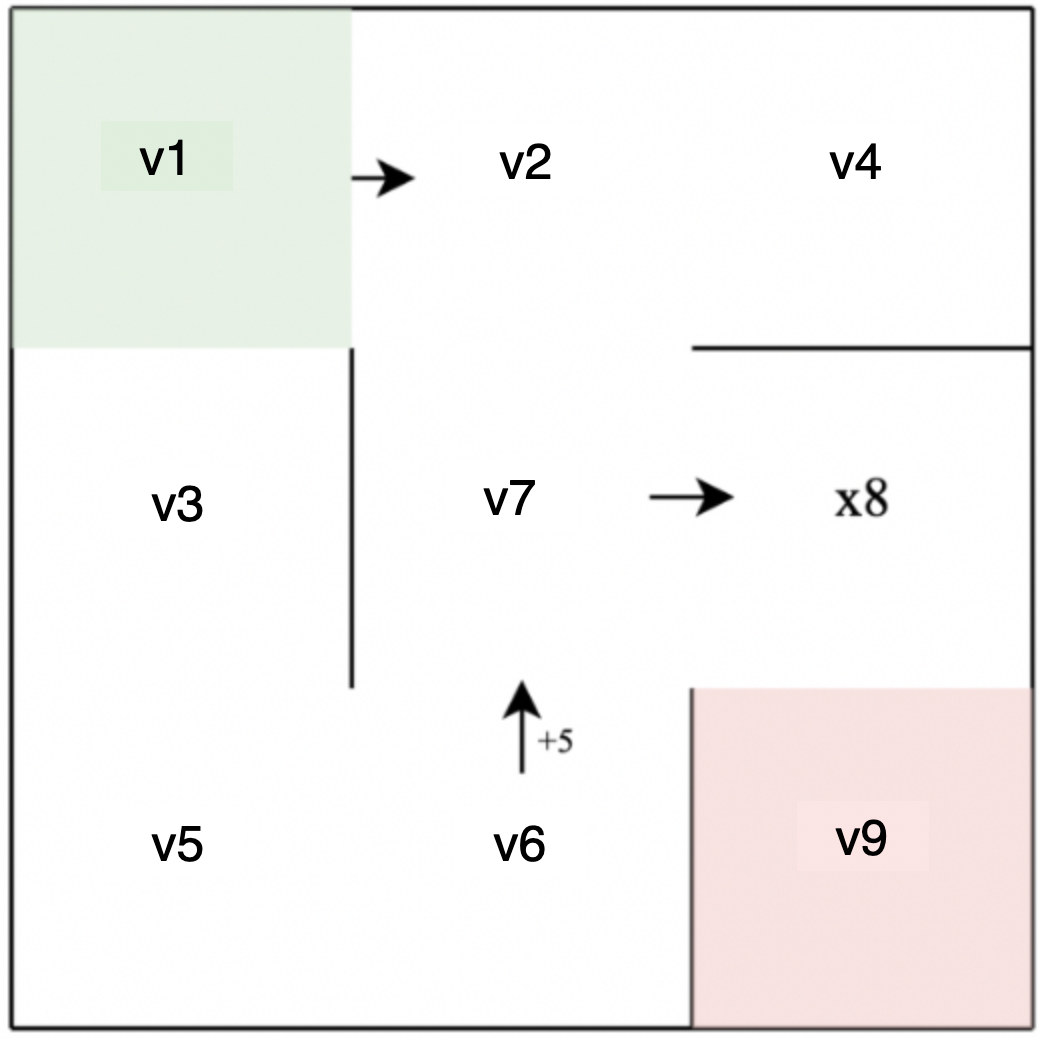
\includegraphics[width=.6\linewidth]{cyclicmaze}
	  \caption{}
	  \label{fig:sub2}
	\end{subfigure}
	\caption{Examples of different mazes. In subfigure (a) an undirected, acyclic maze is shown. In subfigure (b) a maze with a cycle is presented. The maze in subfigure (a) corresponds to the graph in Figure 2.1 (a), and the maze in subfigure (b) corresponds to the graph in Figure 2.1(b). Each cell in a maze is considered as a vertex $v$.\\Source: developed by the author.}
	\label{fig:test}
	\end{figure}	

\begin{definition}\textbf{A Perfect Maze} \emph{is a maze with only one path between any two given nodes.}\end{definition}
\begin{definition}\textbf{An Unperfect Maze} \emph{is a maze with more than one path between any two given nodes.}\end{definition}
 \begin{definition}\textbf{A Texture} \emph{is a general term that refers to the style of the passages of a maze, such as how long they tend to be and which direction they tend to go. Some algorithms will tend to produce mazes that all have similar textures \cite{15}.}\end{definition}
\begin{definition}\textbf{A Canadian Traveller Problem (CTP)} \emph{is a problem of finding the shortest path in a given, known graph with changing conditions in it. The objective of this problem is to find the best solution in the environment which is interfering with malicious intention.}\end{definition}
\begin{definition}\textbf{A Travelling Salesman Problem (TSP)} \emph{is a problem of finding the shortest path between a given list of nodes in the graph.} \end{definition}
\section{Maze Generation Algorithms}
\textcolor{black}{This chapter describes the algorithms that were implemented for this work and were subjected to further comparative analysis. For each algorithm, there is a listing of pseudocode provided along with a picture of the maze generated by it.}
\subsection{Binary Tree}
The Binary Tree algorithm \textcolor{black}{\cite{16}} is the simplest, \textcolor{black}{fast and efficient} algorithm for generating a maze. \textcolor{black}{It does not require a lot of memory because it only needs to remember one cell at any time.} In a given grid, for each cell, algorithm decides whether to carve a passage north or east (or any two other directions south/west, south/east etc. ) between two adjacent cells. The algorithm produces a diagonally biased perfect maze which, in other words, is a random binary tree. For building the whole maze, the algorithm \textcolor{black}{does not} require holding the state of the whole grid. The algorithm only looks at one cell at a time. The time complexity for the Binary Tree generator is $O(|V|)$. \textcolor{black}{A pseudocode for a Binary Tree algorithm is described in Listing 2.1. Examples of mazes produced by this algorithm are presented in Figure 2.5}.
\newline
\begin{lstlisting}[caption={Pseudocode for a Binary Tree Algorithm. Developped by the author, based on ~\cite{16}.}]
\begin{algorithm}
	\FOREACH cell in the grid
		\STATE let neighbours = [];
		\STATE neighbours.push(cell.north);
		\STATE neighbours.push(cell.east);
		\STATE let index = Math.floor(Math.random() * neighbors.length);
		\STATE let neighbor = neighbors[index];
		\STATE cell.link(neighbor);
	\ENDFOREACH	
\end{algorithm}
\end{lstlisting}
\\
\newline
\begin{figure}[!h]
	\centering
	\begin{subfigure}{.45\textwidth}
	  \centering
	  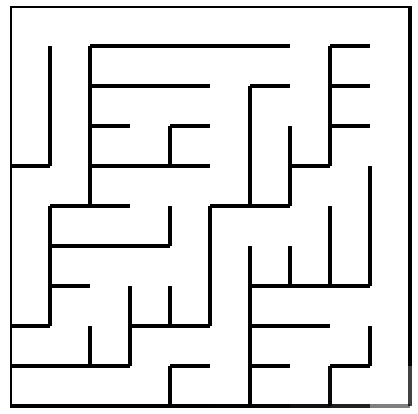
\includegraphics[width=.6\linewidth]{binary1010}
	  \caption{}
	  \label{fig:sub1}
	\end{subfigure}
	\begin{subfigure}{.45\textwidth}
	  \centering
	  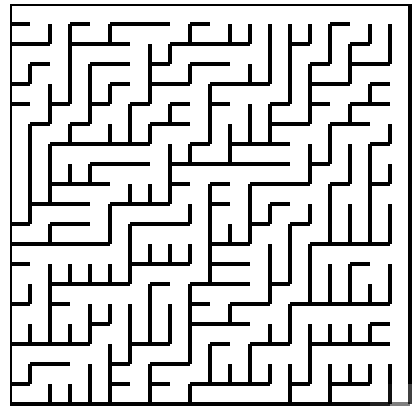
\includegraphics[width=.6\linewidth]{binary2020}
	  \caption{}
	  \label{fig:sub2}
	\end{subfigure}
	\caption{Examples of different mazes generated by the Binary Tree algorithm implemented for this work. In subfigure (a) a maze of size 10 $\times$ 10, and in subfigure (b) of size 20 $\times$ 20.\\Source: developed by the author.}
	\label{fig:test}
	\end{figure}
\newline
\\
\\
\\
\newpage
\subsection{Aldous-Broder}
The Aldous-Broder is a well-known algorithm for generating uniform spanning trees (USTs) based on random walks. This means that the maze is perfect and
unbiased~\cite{17}. The algorithm is highly inefficient but does not require a lot of memory. In a given grid, the algorithm randomly chooses any cell,
and for this cell randomly chooses a neighbour and if this neighbour was not previously visited, the algorithm links it to the prior cell. It is repeated
until every cell has been visited. To build a spanning tree, the random walk needs to visit every vertex of the graph at least once. The time complexity
for the Aldous-Broder generator is $O(|V|^3)$. In Listing 2.2 the pseudocode for an Aldous-Broder algorithm is described. Examples of mazes produced by
this algorithm are presented in Figure 2.6.
\newline
\begin{lstlisting}[caption={Pseudocode for an Aldous-Broder algorithm. Developped by the author, based on~\cite{17}.}]
\begin{algorithm}
	\STATE let cell = grid.get_random_cell();
	\WHILE unvisited cell in the grid
		\STATE let neighbours = cell.neighbours
		\STATE let index = Math.floor(Math.random() * neighbours.length);
		\STATE let neighbour = neighbours[index];
		\IF neighbour has no links
			\STATE cell.link(neighbour);
		\ENDIF
		\STATE cell = neighbour;
	\ENDWHILE
\end{algorithm}
\end{lstlisting}

\newline
\begin{figure}[!h]
	\centering
	\begin{subfigure}{.45\textwidth}
	  \centering
	  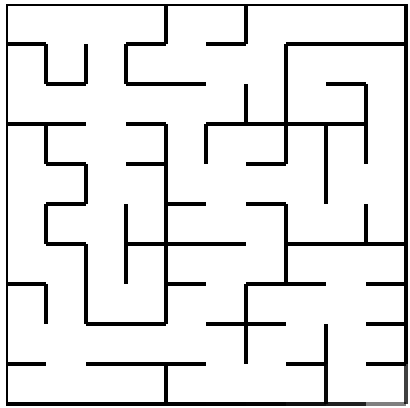
\includegraphics[width=.6\linewidth]{aldous1010}
	  \caption{}
	  \label{fig:sub1}
	\end{subfigure}
	\begin{subfigure}{.45\textwidth}
	  \centering
	  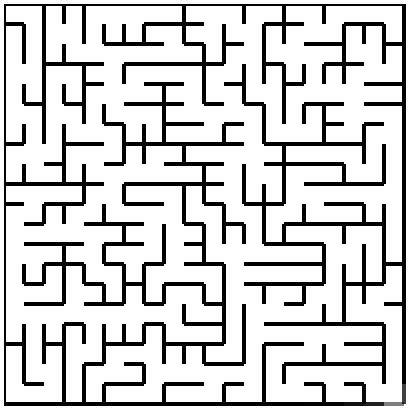
\includegraphics[width=.6\linewidth]{aldous2020}
	  \caption{}
	  \label{fig:sub2}
	\end{subfigure}
	\caption{Examples of different mazes generated by the Aldous-Broder algorithm implemented for this work.
	In subfigure (a) a maze of size 10 $\times$ 10, and in subfigure (b) of size 20 $\times$ 20.\\Source: developed by the author.}
	\label{fig:test}
	\end{figure}
\newpage
\subsection{Recursive-Backtracker}
The Recursive Backtracker is one of the Depth First Search algorithm (DFS) which may be also used for generating mazes. It generates perfect mazes with a
small ratio of dead-ends in a maze. Its main disadvantage is that it requires a lot of memory, so it is not fast or efficient\cite{18}.
The algorithm starts at the randomly selected cell and carves its way until it must “turn around” and backtracks to the nearest “not carved yet” cell.
This process continues until it discovers all the vertices that are reachable from the source vertex. The time complexity for the Recursive-Backtracker
generator is $O(|V|+|E|)$. In Listing 2.3 the pseudocode for a Recursive Backtracker algorithm is described. Examples of mazes produced by this algorithm
are presented in Figure 2.7.

\begin{lstlisting}[caption={Pseudocode for a Recursive-Backtracker algorithm. Source: developped by the author, based on~\cite{18}.}]
	\begin{algorithm}
		\STATE let cell = grid.get_random_cell();
		\STATE let stack = [cell]
		\WHILE stack.length > 0
		\STATE let current_cell = stack[stack.length - 1];
		\STATE let neighbors = current.neighbors();
			\IF neighbors.length == 0
				\STATE stack.pop()
			\ELSE 
				\STATE let neighbor = neighbors[Random]
			\STATE current.make_link(neighbor)
			\STATE stack.push(neighbour)	
	\end{algorithm}
	\end{lstlisting}
\newline
\begin{figure}[!h]
    \centering
    \begin{subfigure}{.45\textwidth}
    \centering
    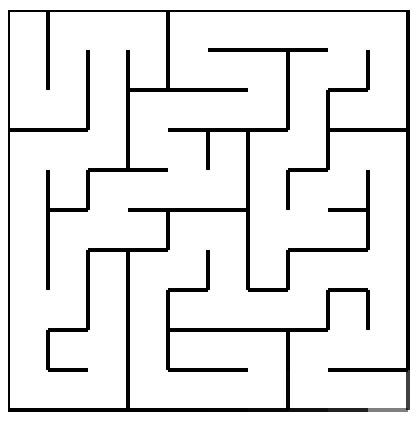
\includegraphics[width=.6\linewidth]{recursive1010.png}
    \caption{}
    \label{fig:sub1}
    \end{subfigure}
    \begin{subfigure}{.45\textwidth}
    \centering
    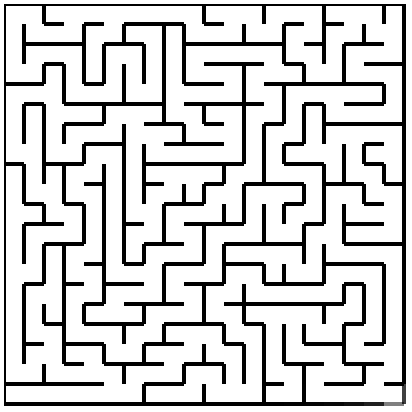
\includegraphics[width=.6\linewidth]{recursive2020.png}
    \caption{}
    \label{fig:sub2}
    \end{subfigure}
    \caption{Examples of different mazes generated by the Recursive Backtracker algorithm implemented for this work.
	In subfigure (a) a maze of size 10 $\times$ 10, and in subfigure (b) of size 20 $\times$ 20.\\ Source: developed by the author.}
    \label{fig:test}
    \end{figure}
\section{Maze Solving Algorithms}
\subsection{Breadth-First Search Algorithm}
BFS is one of the simplest algorithms for searching a graph. As already mentioned, each maze may be considered as a graph, so from now on we will call 
BFS  a solving algorithm or simply a solver of a given maze. From graph theory, we can state that for a given graph $ G = ( V, E) $, and distinct source 
vertex $p$, BFS explores the edges of $G$ to ,,visit’ each vertex directly connected with $p$. The algorithm also produces a BFS tree with $p$ root that 
contains all reachable vertexes. The shortest path between $p$ and any vertex $v$ in $G$ is a simple path in the BFS tree, that is, a path containing
the smallest number of edges~\cite{16}. The BFS implemented in this work is described in Listing 2.4.\newline
\begin{lstlisting}[caption={Pseudocode for a BFS algorithm. Source: developped by the author, based on~\cite{16}.}]
	\begin{algorithm}
		\STATE let stack = new Array();
		\STATE stack.push(maze.startcell);
		\STATE let currentcell = startcell;
		\WHILE (!finished){
			STATE let cellAdjacents = grid.getAdjacents(currentcell);
			\FOR EACH cell in cellAdjacents{
				\IF cell == !visited{
					\STATE cell == visited;
					\STATE cell.parent = current;
					\STATE stack.push(cell);
				}
			}
			\STATE current = stack.pop();
		}
	\end{algorithm}	
\end{lstlisting}	

\subsection{Dijkstra Algorithm}
Dijkstra is a solving algorithm for single-source shortest-path problems. We can apply it on a directed graph $G=(V, E)$ with a constraint of no negative edges. 
It repeatedly chooses the closest vertex in $V-S$ to add to set S. 
Where \textit{S} is a set of vertices whose final shortest-path weights from the source \textit{p} have already been determined.
The algorithm floods the graph so it uses a greedy strategy. The Dijkstra Algorithm implemented in this work is described in Listing 2.5.\\
\begin{lstlisting}[caption={Pseudocode for a Dijkstra’s algorithm.Source: developped by the author, based on~\cite{18}.}]
	\begin{algorithm}
		\STATE let distances = new Distances();
		\STATE let frontier = new Array();
		\WHILE unvisited cell in the grid
		\FOREACH linked cell in frontier
			\STATE linked_cell.distance = cell.distance +1;
			\STATE distances.set_cell(linked_cell);
			\STATE frontier.push(linked_cell);
	    \ENDFOREACH
	\RETURN distances;
	\end{algorithm}
	\end{lstlisting}

\subsection{A* Algorithm}
$A^*$ algorithm is one of the most powerful path-finding algorithms. It uses the same functions derived from the previously described Dijkstra Algorithm. 
$A^*$ combines the information that Dijkstra’s Algorithm uses, meaning choosing the vertex which is close to the starting point and additionally
implementing a new type of information, which is heuristic. That means choosing nodes which are estimated to be close to the ending point $q$. 
In the standard terminology used when considering A*, $g(v)$ represents the exact cost of the path from the starting point $p$ to any vertex $v$, and
$h(v)$ given by equation (2.5) describes the heuristic estimated cost from vertex $v$ to the goal $q$. In each loop, the algorithm minimizes the function
$f(n)$ given by equation (2.4). The $A^*$ Algorithm implemented in this work is described in Listing 2.6.
\begin{equation}
f(n) = g(v) + h(v)
\end{equation}
\textbf{Where:}\\
$g(v)= |v - p| + |v - n|$\\
$|v - p|$ it is a distance from the starting point $p$ to any current vertex $v$\\
$|v - n|$ it is a distance from any current vertex $v$ to its neighbour $n$.\\
\newline
The heuristic cost from neighbour vertex $v$ to goal vertex $q$ is given as a:
\begin{equation}
h(v) = |q.x - n.x| + |q.y - n.y|
\end{equation}
\textbf{Where:}\\
$x$ and $y$ are grid coordinates of vertices\\

\begin{lstlisting}[caption={Pseudocode for a A* algorithm. Source: developped by the author, based on~\cite{19}.}]
	\begin{algorithm}
		\STATE let openlist = new Array();
		\STATE let closelist = new Array();
		\STATE let startcell = maze.startcell;
		\STATE let goalcell = maze.goalcell;
		\STATE startcell.set_g_score();
		\STATE startcell.set_f_score();
		\STATE openlist.push(startcell)
		\STATE let finished = false;
		\WHILE (!finished)
			\STATE let currentcell = openlist    
			.find_cell_with_lowest_fvalue();
			\STATE let neighbours = currentcell.get_links();
			\IF currentcell == goalcell
				finished = true;
				closelist.push(currentcell);
			\ELSE 
			\FOREACH neighbour => neighbours	
			\IF inEitherList(openlist, closelist)
				\STATE g_score = calulate_gscore(cell);
				\STATE f_score = calculate_fscore(cell);
				\STATE parent = setParent(cell);
				\STATE openlist.push(cell)
			\ENDIF
			closelist.push(currentcell);
			openlist.remove(currentcell);
	    	\ENDFOREACH
	\end{algorithm}
	\end{lstlisting}
%